\documentclass{article}
\usepackage{graphicx}
\graphicspath{{./images/}}
\usepackage{geometry}
\usepackage{hyperref}
\usepackage{paralist}
\usepackage[round]{natbib}
\usepackage{sectsty}
\usepackage{gensymb}
\usepackage{caption}
\usepackage{subcaption}
\usepackage{listings}
\usepackage[space]{grffile}
\usepackage{latexsym}
\usepackage{amsfonts,amsmath,amssymb}
\usepackage{url}
%\usepackage{minitoc}
\hypersetup{colorlinks=false,pdfborder={0 0 0}}
\usepackage{textcomp}
\usepackage{longtable}
\usepackage{multirow,booktabs}
\newcommand{\truncateit}[1]{\truncate{0.8\textwidth}{#1}}
\newcommand{\scititle}[1]{\title[\truncateit{#1}]{#1}} 
\usepackage[parfill]{parskip}

% Typeface
\usepackage{ifxetex}
\ifxetex
  \usepackage{fontspec}
  \defaultfontfeatures{Ligatures=TeX} % To support LaTeX quoting style
  \setmainfont[Mapping=tex-text, Color=textcolor]{HelveticaNeue}
  %\setmainfont[Mapping=tex-text, Color=textcolor]{Avenir LT Std}
\else
  \usepackage[T1]{fontenc}
  \usepackage[utf8]{inputenc}
  \renewcommand{\familydefault}{\sfdefault}
  \usepackage{helvet}
\fi
%\chapterfont{\Large} % \sffamily
%\renewcommand{\chaptername}{}
%\renewcommand{\thechapter}{}

% Title page
\usepackage{xcolor}
\definecolor{titlepagecolor}{cmyk}{0,0,0,0}
\definecolor{namecolor}{cmyk}{0,0,0,1} 
\definecolor{chaptertitlepagecolor}{cmyk}{0,0,0,0.9}
\definecolor{chapternamecolor}{cmyk}{0,0,0,0.3}  

\begin{document}

%---------------------------------------------- BODY ----------------------------------------------

\section{Tangible engagement}

\subsection{Introduction}

Theoretically tangible interfaces for geographic information systems (GIS) have the potential to
radically transform the role of stakeholders in 
environmental issues. 
%
GIS have geospatial analyses, models, and simulations 
needed to scientifically study and predict a wide array of interacting environmental processes. 
%
Given the complexity of parameterizing spatial algorithms and working with multi-dimensional data, 
GIS, however, can be challenging to learn and use \citep{Ratti2004}.
%
If GIS felt so natural to use that stakeholders without any computing experience could use a GIS to explore environmental processes 
then stakeholders could drive environmental decision-making,
radically opening science, design, and management (if political will allowed). 
%

These theses have yet to be demonstrated and proven. 
The effectiveness of tangible interfaces like shape displays need to be empirically tested \citep{Rasmussen2012}. 
The ways in which tangible geospatial modeling mediates learning and thinking about processes should to be studied. 
The effectiveness of engaging stakeholder should to be demonstrated in diverse contexts. 
A real-world demonstration of stakeholders using tangible geospatial modeling to solve a set of complex environmental problems, 
alone,
would not be enough to understand how and why the process works -- if it does -- and how it could be improved. 
Experimental studies in the lab, user studies in the field, and real-world implementation should be coupled with the continued design and development of the technology.


\subsection{The importance of engagement}

Both pragmatically and ethically
it is important to engage those involved in environmental issues like biodiversity conservation. 
%
Without engaging those involved 
efforts to solve complex environmental problems like the loss of biodiversity may be ineffectual and will certainly be unjust.
%
%Reserves designed to exclude local people, 
%reserves that ignore local socio-cultural realities
%are likely to fail without intensive management, continued political will, and adequate resources. 
%
Top-down planning and command-and-control governance has led to the establishment 
of ineffective conservation reserves in developing nations, to `paper parks' 
such as Sierra Chinaj\'{a} in Quatemala which is threatened by land invasion and resource extraction 
\citep{Bonham2008}. 
%
Citing the inequitable distribution of land and the insecurity of land tenures 
as the underlying drivers of biodiversity loss in Sierra Chinaj\'{a}
\citeauthor{Bonham2008} argue that engaging local people rather than excluding them 
could transform ``squatters' to `stewards'' \citeyearpar{Bonham2008}. 
%
To foster local stewardship 
\citeauthor{Brosius2003} advocate indigenous management in conservation reserves 
and the devolution of power to local stakeholders 
\citeyearpar{Brosius2003}.
%
\citeauthor{Brosius2003} also question the validity, legitimacy, and justice of maps made by 
` governments, industry, and local elites' 
which fail to incorporate local knowledge, values, and interests 
\citeyearpar{Brosius2003}.
%
How can local knowledge be included in maps, models, and simulations? 

\subsection{Open science}
Open science strives for accessibility, transparency, and reproducibility
through open access, open data \citep{Boulton2012}, 
free and open source software \citep{Ince2012,Rocchini2012}, and
open education \citep{Petras2015}. 
% why?
When science is accessible, transparent, and reproducible 
it is more inclusive, more critical, and thus more legitimate. 
%
The scientific community needs access to research and data in order to reproduce it -- in order to test and validate it. 
%Science gains legitimacy -- acceptance -- when it is reproducible. 
The research process should be more transparent so that 
algorithms, experiments, and data can be scrutinized, reproduced, tested, and critiqued. 
Theoretically this could fuel the pace of scientific research, lower the cost of research, and build scientific credibility. 
Open science projects like the Nutrient Network, a grassroots ecological monitoring network, 
have already delivered rapid and cost effective results \citep{Stokstad2011}. 

Open science calls for a culture of openness, collaboration, and inclusion
that could potentially engage a much broader community 
by encouraging for example citizen science. 
%
In a truly open science
models would be so open that stakeholders could co-develop them
and make them their own. 
%
% co-modeling
By collaboratively developing scientific models 
with local stakeholders, scientists can 
`redistribute expertise' 
and collectively generate new knowledge \citep{Whatmore2011, Landstrom2011}. 
%
With a series of case studies 
\citeauthor{Sandker2010} show
that participatory modeling can 
encourage strategic thinking across disciplines, 
highlight underlying drivers of change, 
and identify trade-offs,
but also caution against overly complex models
, arguing for 
`a balance between `models as stories' and technical
modeling'
\citeyearpar{Sandker2010}.  
%

% data collection
Local stakeholders can also be engaged in and empowered by the collection of open data. 
%
In Participatory 3D Modeling stakeholders such as indigenous communities 
map 
geographic features, resources, practices, and rights 
on a physical 3D contour model 
using familiar, everyday materials such as pins, yarn, and paint 
to share their traditional spatial knowledge. 
The 3D model helps situate stakeholders in space in an intuitive way
and the familiar media are natural to use as they draw on existing skills.
The tangible quality of the physical model and material traces of their mapping 
promote a sense of agency and ownership. 
%
The completed model is digitized, stored, and mapped in a GIS. 
The physical 3D model and prints of digital maps are left with the community
as a resource for
education, communication, resource management, establishing land rights, and conflict resolution 
\citep{Rambaldi2001}.
%
The Forage Tracking project, another example of participatory mapping, helped a cooperative of catadores -- informal recyclers -- 
in S\~{a}o Paulo to track and map their routes.
%
With the help of the researchers the cooperative mapped their routes using GPS tracking and real-time web mapping.
They also collaboratively designed a software platform for community recycling 
through a participatory process that highlighted the need for trust in the community. 
By mapping the informal recyclers' routes 
the project helped to establish 
`a sense of identity for the cooperative,
providing tangible evidence of their place in the city.'
\citep{mit2012,Offenhuber2012}.
%

%%%%%%%%%%%%%%%%%%%%%%%
\subsection{Tangibles}
% vision

Technology can play an important role in engaging stakeholders. 
Technology can help stakeholders collect data, 
collaboratively design and develop scientific models, 
and explore scenarios.
%
% tangibles
Tangibles -- technologies that interactively, physically manifest the digital -- are designed to make interaction with computers more natural and intuitive. Tangibles could make technology much more accessible to stakeholders with limited or no experience with computers. 
% tangible programming  
Tangible programming \citep{Horn2007} could potentially be used to engage stakeholders more deeply in the development of scientific models.  
% tangible interfaces
Tangible interfaces for geographic information systems like Tangible Landscape \citep{Petrasova2015} could, theoretically, 
enable stakeholders to naturally interact with complex geospatial models and simulations in order to develop and explore scenarios without any computer experience. 
%

%
A tangible interface using familiar, everyday materials in everyday ways should be natural to interact with 
because it leverages existing sensorimotor schemas. 
%
When interactions are analogous to everyday tasks 
the user subconsciously knows what to do and how to do it. 
%
In tangibles materiality -- the feel, look, and physics -- of the media used matters. 
The choice of material can afford different interactions
and mediate meaning, emotion, and motivation. 
%


% scale
% ...

% coffee and viz
We hosted a participatory modeling workshop using Tangible Landscape 
as part of North Carolina State University Library's Coffee \& Viz series \citep{Harmon2016}. 
%
In this interactive seminar participants 
explored complex environmental problems 
by playing serious games. 
%
In the games
participants used simple tangible interactions 
to computationally steer simulations, 
to drive simulated environmental processes. 
%
In one game participants managed the spread of termites across a city by treating city blocks. 
To treat a city block they placed wooden cubes representing preventive treatments on the game board 
leveraging basic motor skills from childhood play 
(Fig.~\ref{fig:termite_game}).
%
In the other game participants tried to save houses from coastal flooding by building coastal defenses. 
To build defenses they sculpted dunes out of polymeric sand
again leveraging motor skills from childhood play
(Fig.~\ref{fig:coastal_game}). 
%
Participants were able to naturally 
interact with a statistical epidemiological model 
and a flood simulation. 
Because the interactions were so simple % yet afforded so much
they were able to iteratively 
explore the behavior of multidimensional environmental processes
unfolding in time and space. 

% images: termites and coastal

\begin{figure}
        \centering
        \begin{subfigure}[t]{0.3\textwidth}
                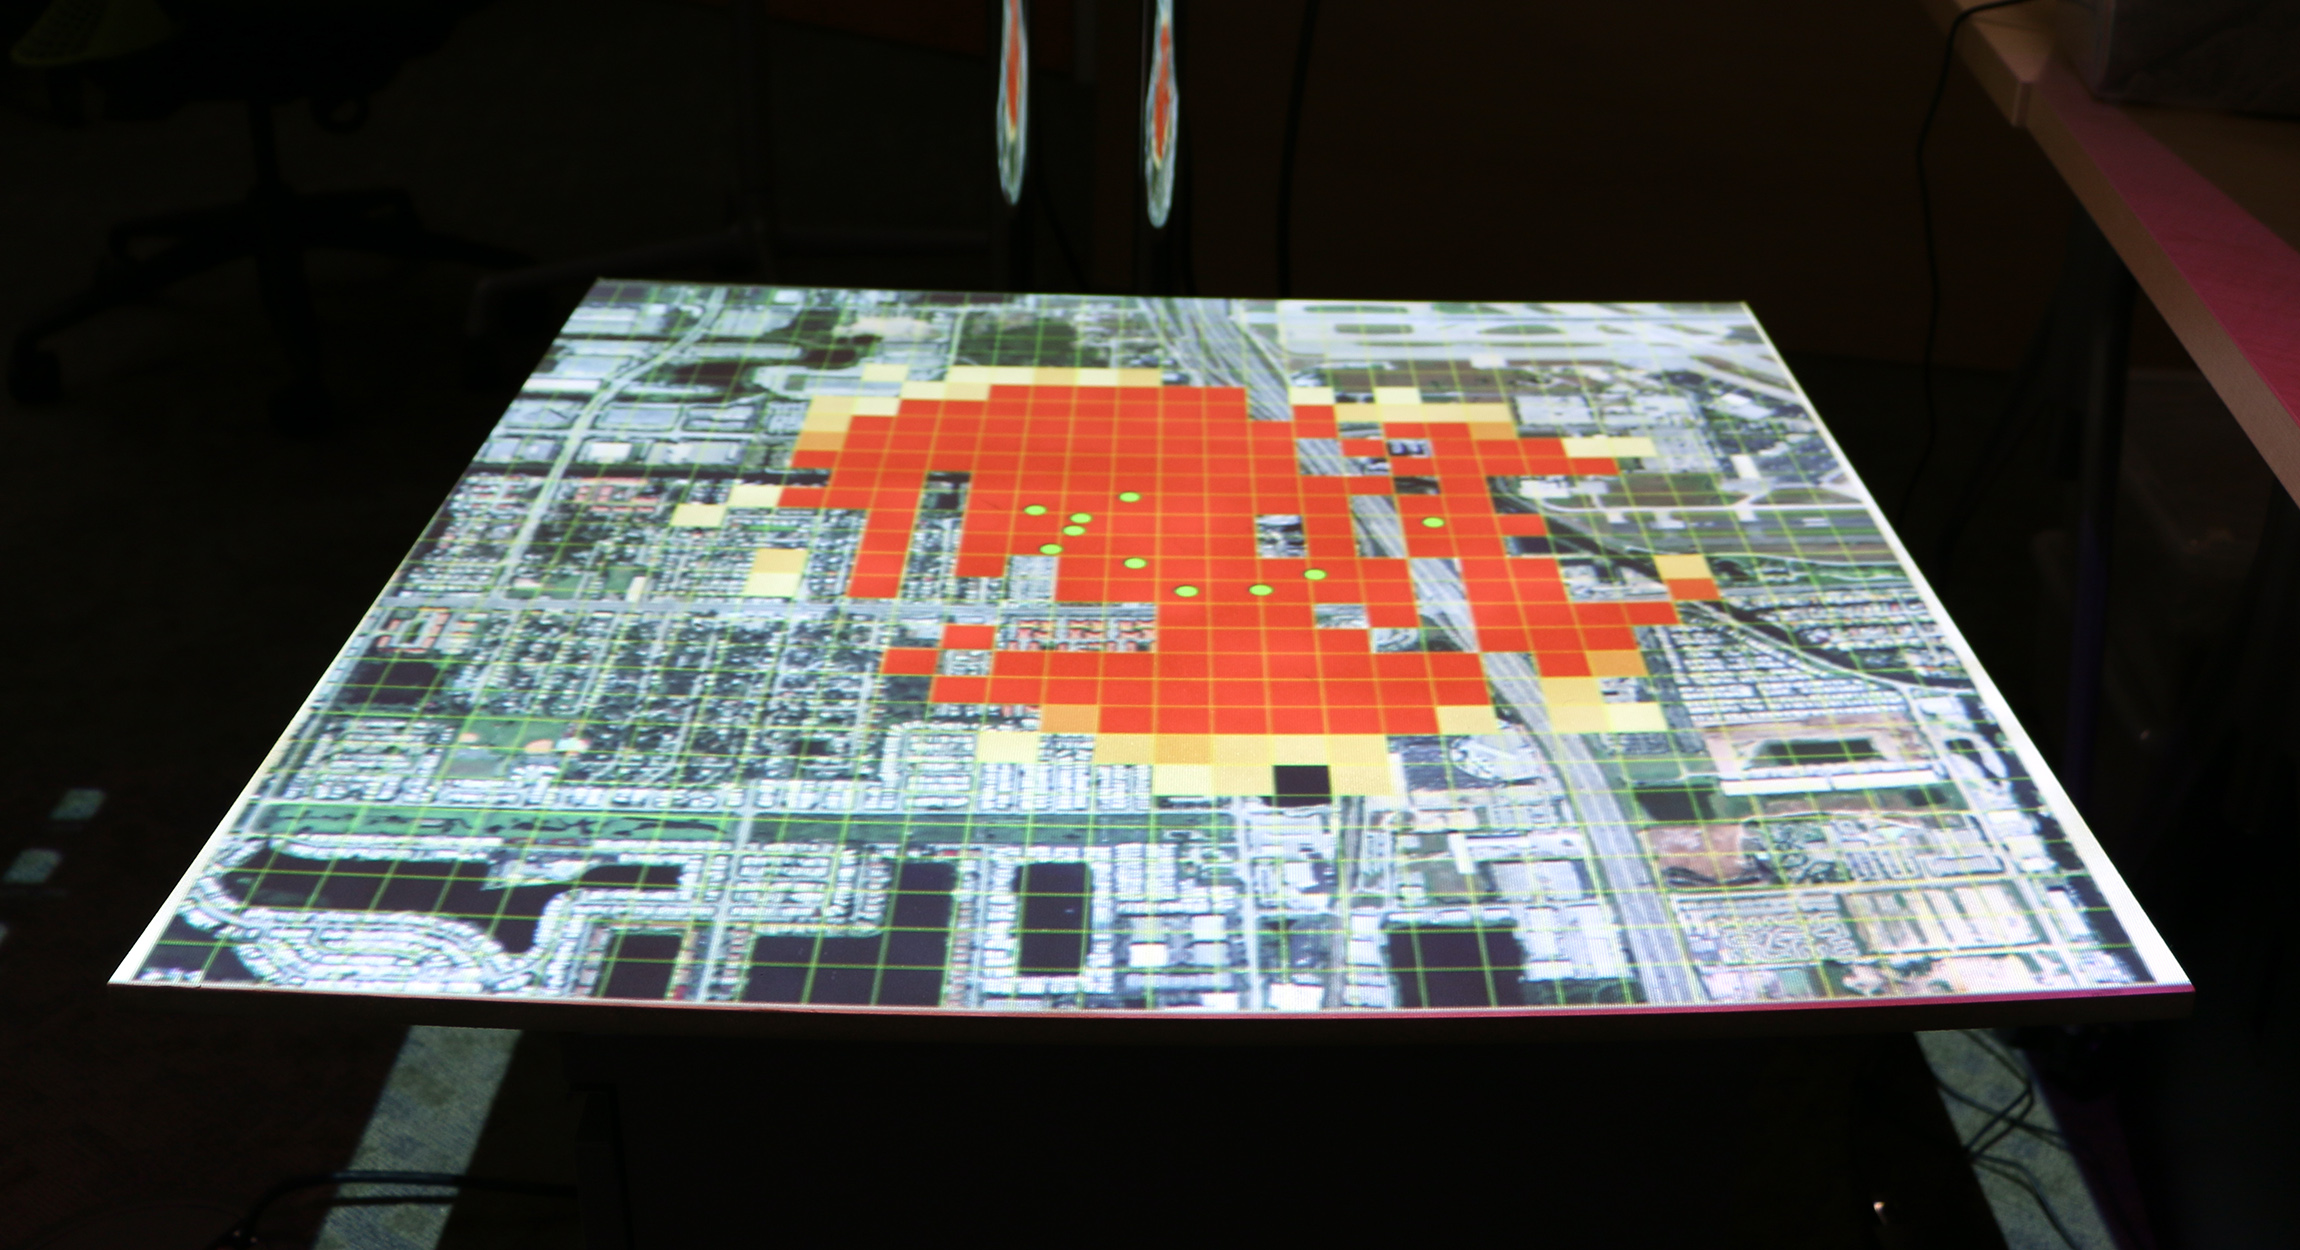
\includegraphics[trim={0 0 0 1cm},clip,width=\textwidth]{termite_game_1}
                %\caption{The initial simulated spread of termites across Dania Beach, Florida}
        \end{subfigure}
        ~ %add desired spacing between images, e. g. ~, \quad, \qquad, \hfill etc.
        \begin{subfigure}[t]{0.3\textwidth}
                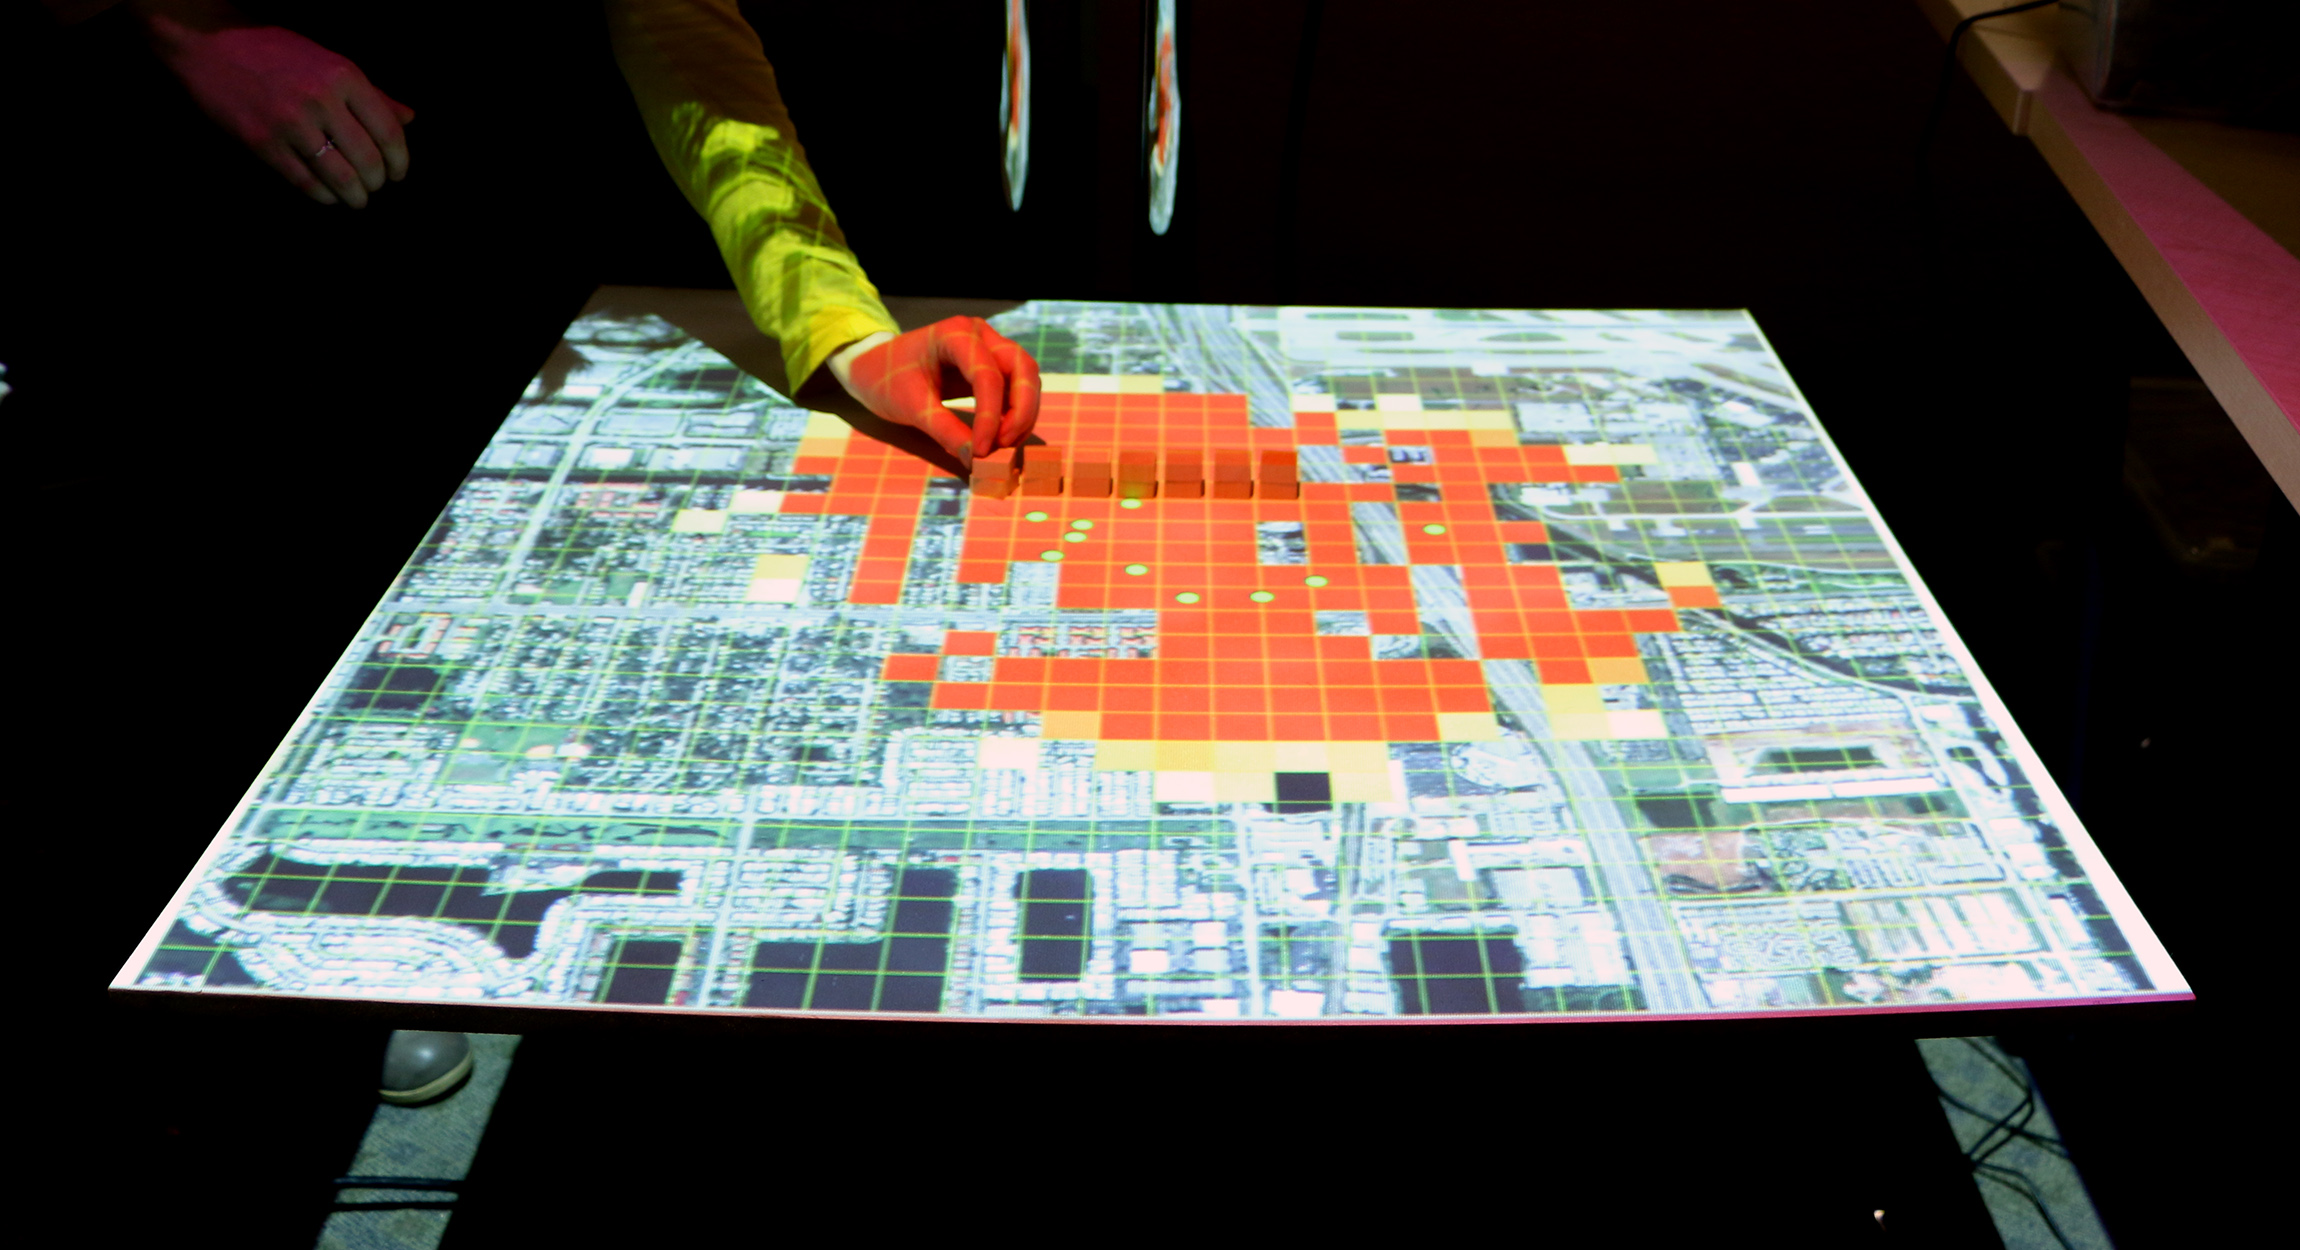
\includegraphics[trim={0 0 0 1cm},clip,width=\textwidth]{termite_game_2}
                %\caption{A participant places a wooden cube to treat a city block}
        \end{subfigure}
        ~ %add desired spacing between images, e. g. ~, \quad, \qquad, \hfill etc.
        \begin{subfigure}[t]{0.3\textwidth}
                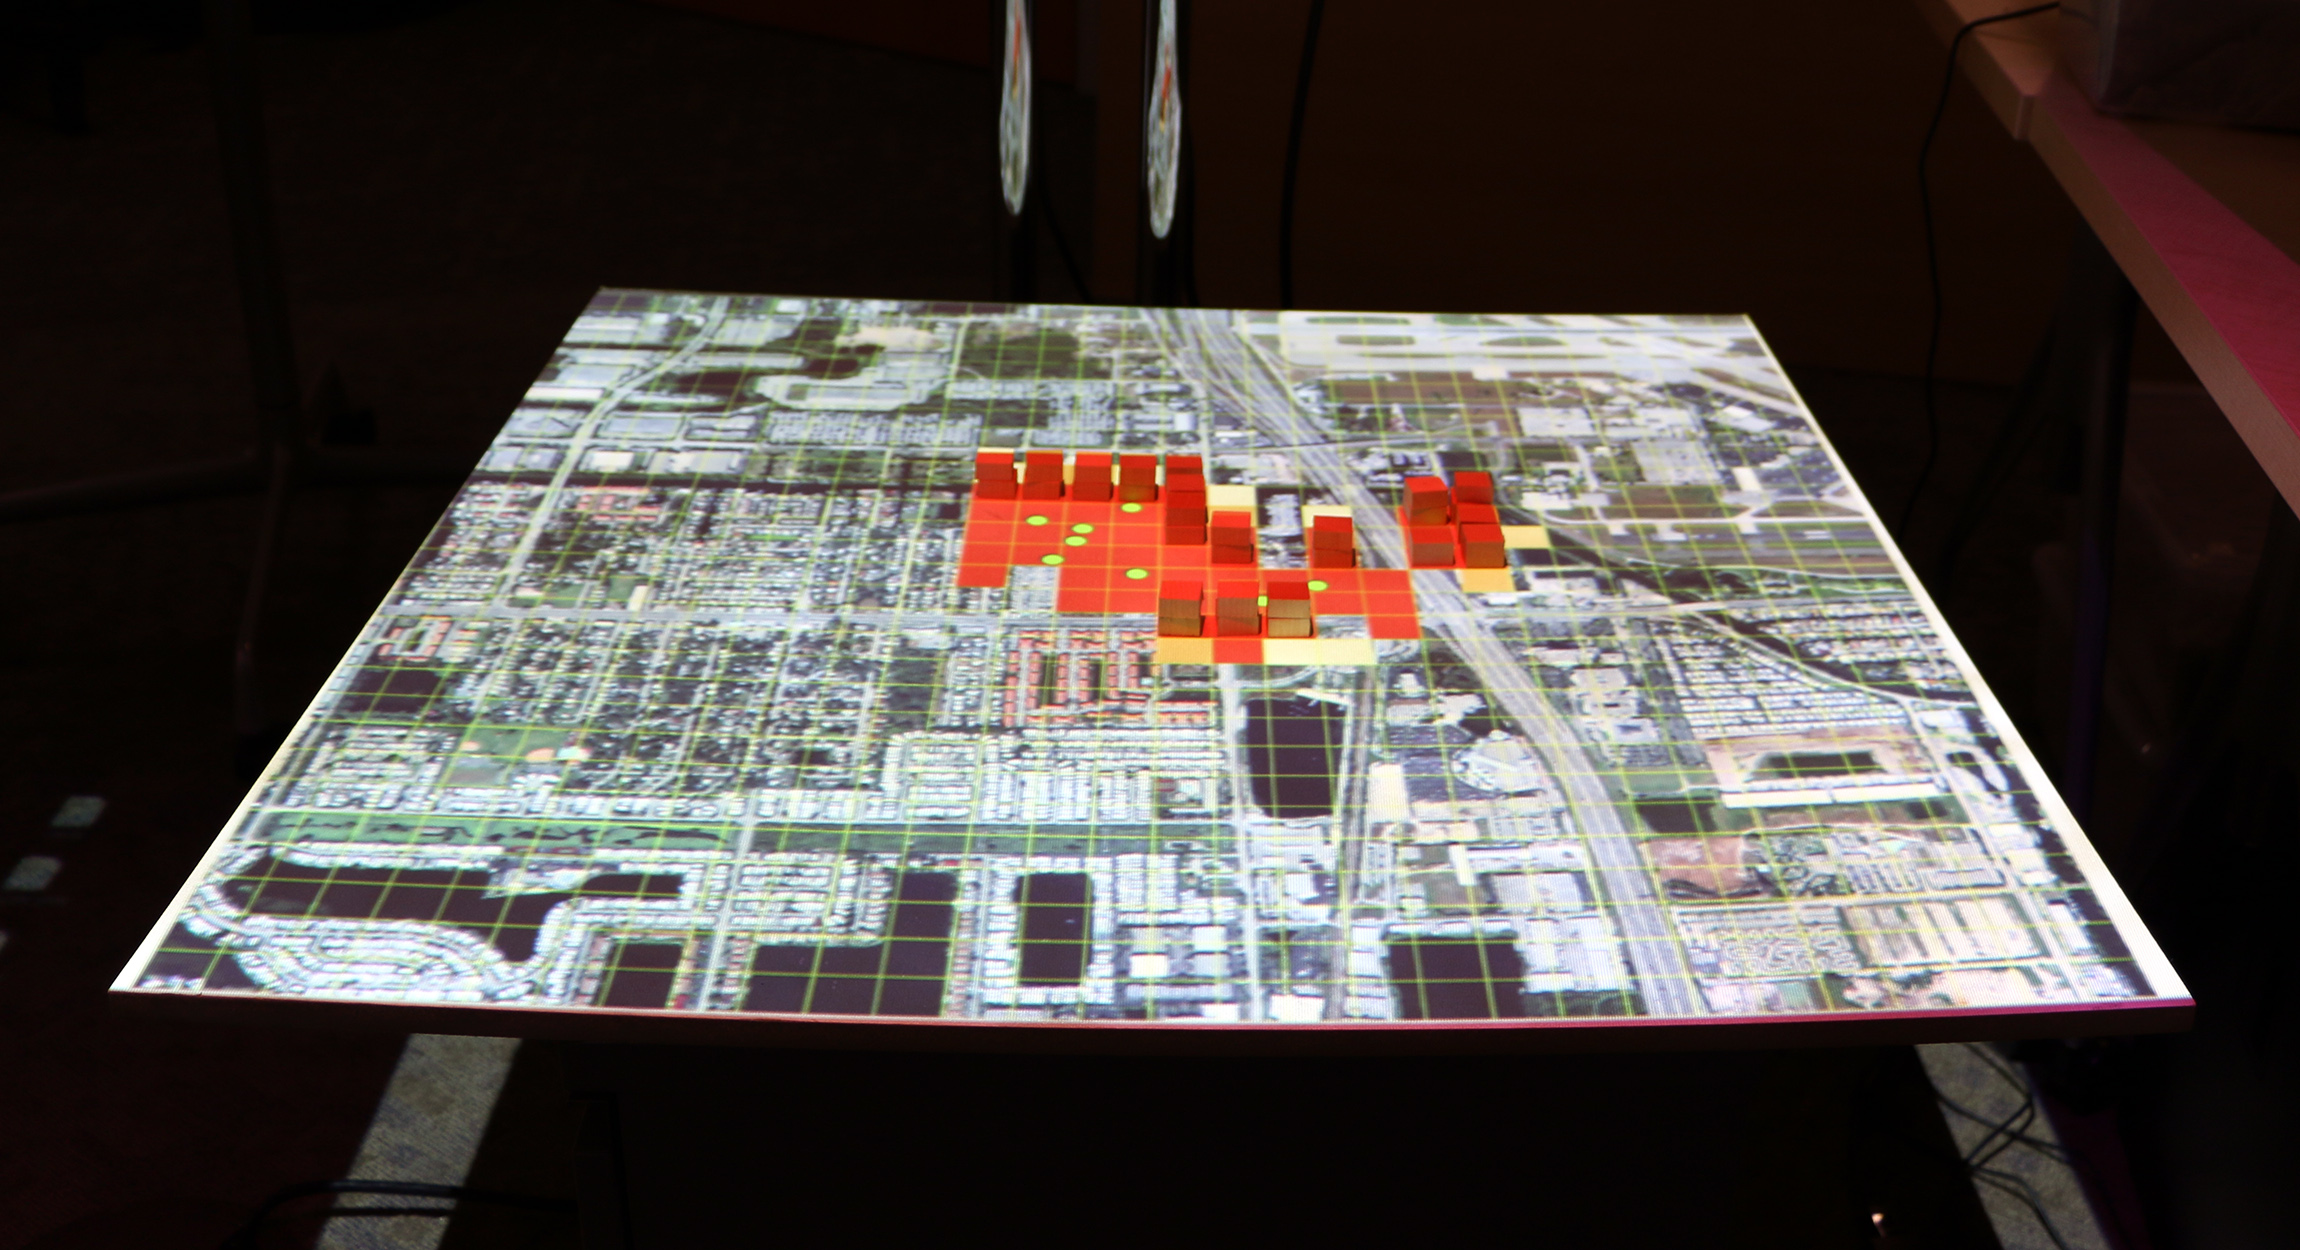
\includegraphics[trim={0 0 0 1cm},clip,width=\textwidth]{termite_game_3}
                %\caption{The simulated spread of termites after preventative treatment}
        \end{subfigure}
        \caption{Serious gaming with Tangible Landscape: the termite spread game}
        \label{fig:termite_game}
\end{figure}

\begin{figure}
        \centering
        \begin{subfigure}[t]{0.225\textwidth}
                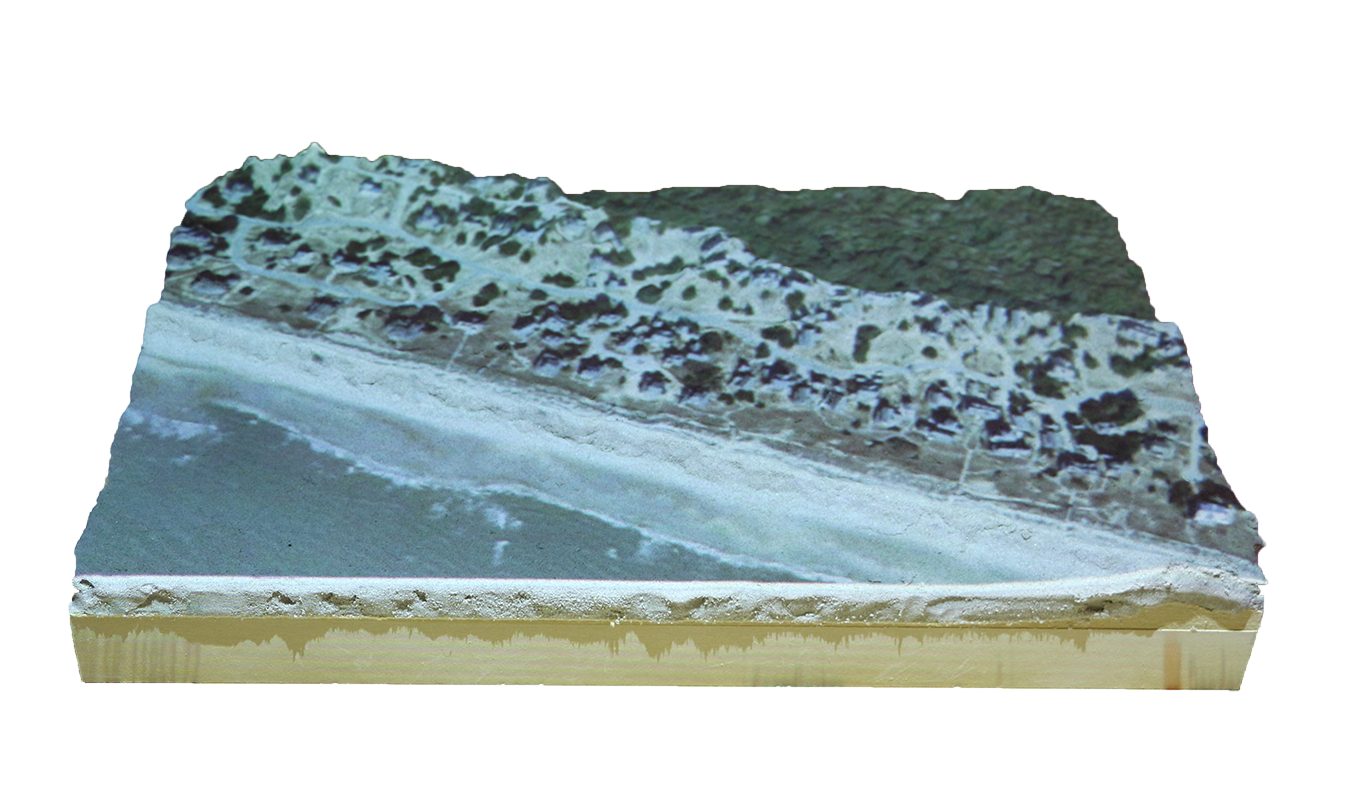
\includegraphics[trim={0 0 0 1cm},clip,width=\textwidth]{tl_coastal_1s.png}
                %\caption{A model of a vulnerable beach on Bald Head Island}
        \end{subfigure}
        ~ %add desired spacing between images, e. g. ~, \quad, \qquad, \hfill etc.
        \begin{subfigure}[t]{0.225\textwidth}
                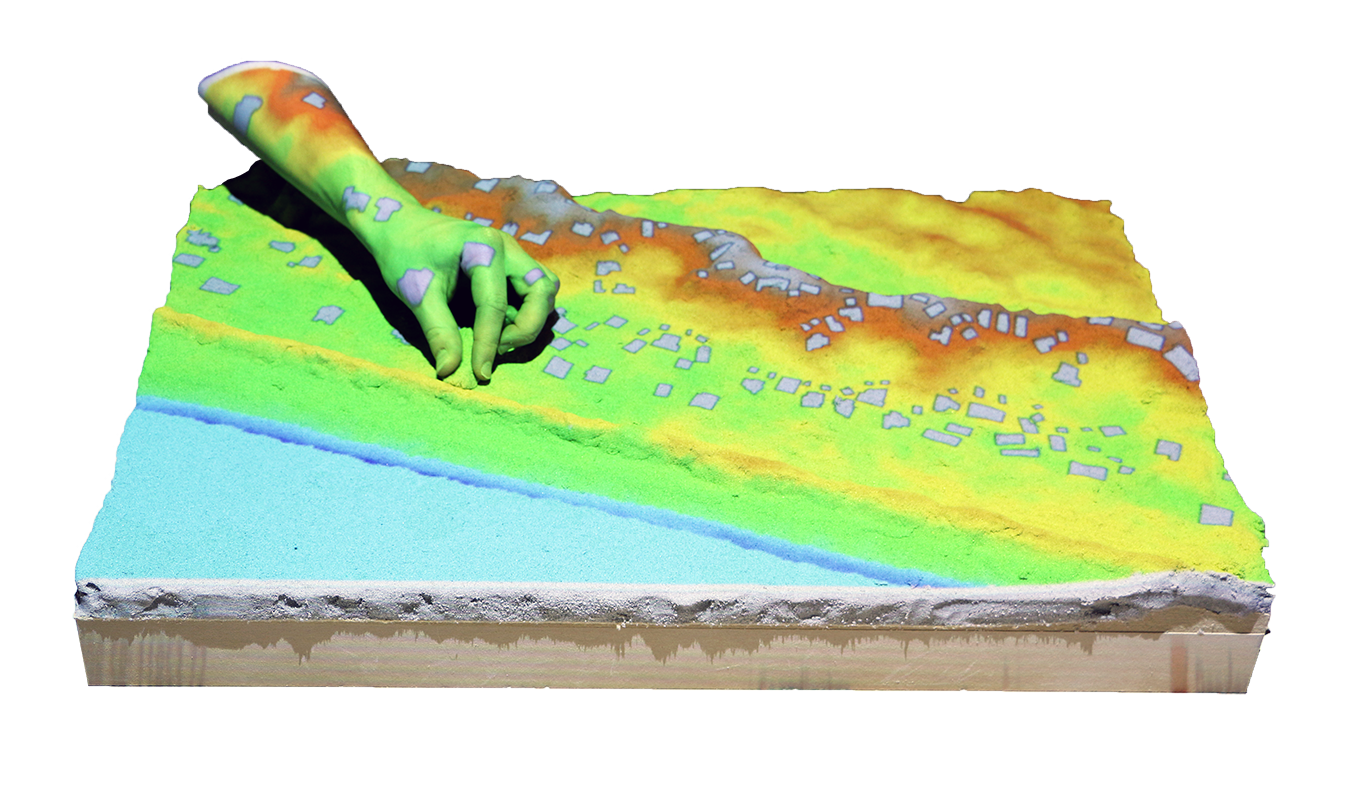
\includegraphics[trim={0 0 0 1cm},clip,width=\textwidth]{tl_coastal_2s.png}
                %\caption{Players build flood defenses using their sand budget}
        \end{subfigure}
        ~ %add desired spacing between images, e. g. ~, \quad, \qquad, \hfill etc.
        \begin{subfigure}[t]{0.225\textwidth}
                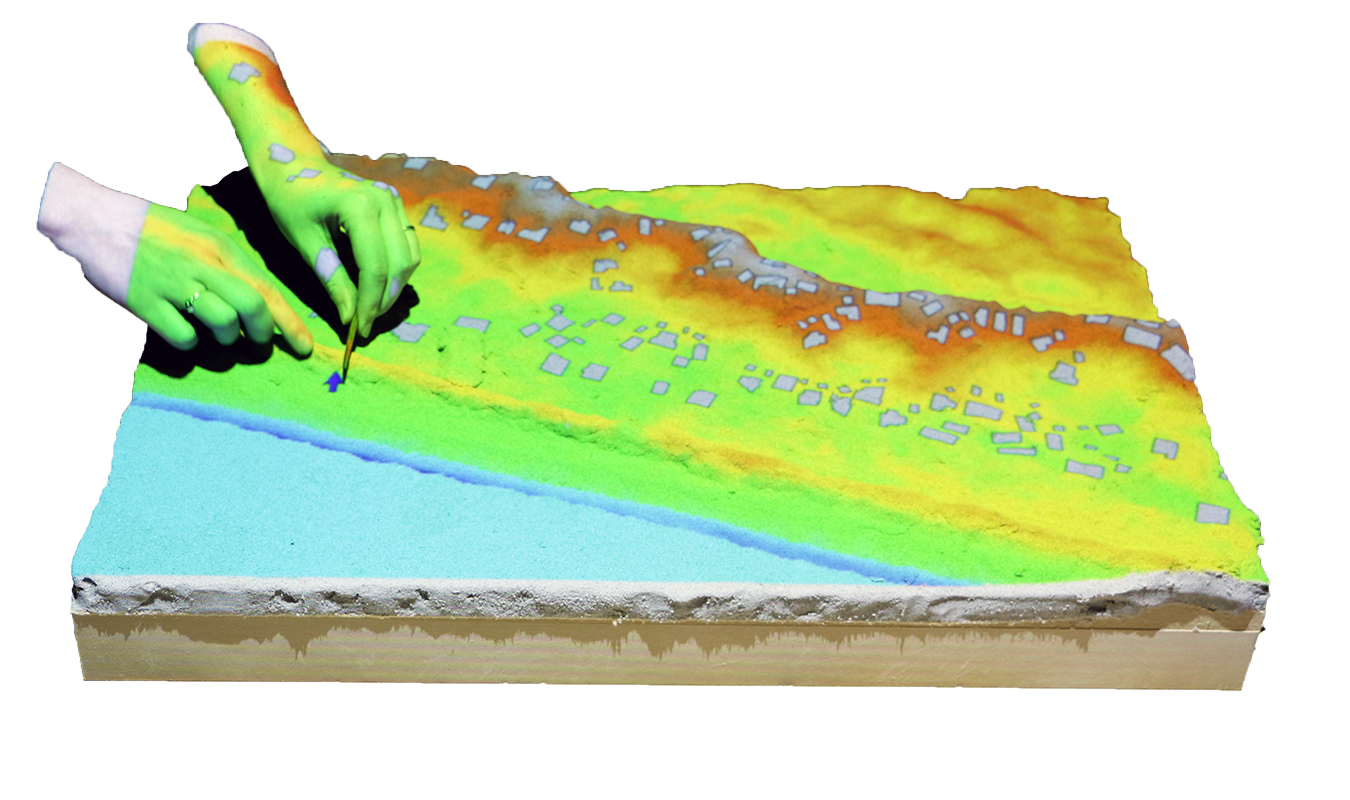
\includegraphics[trim={0 0 0 1cm},clip,width=\textwidth]{tl_coastal_3s.png}
                %\caption{The game master breaches the dune at a random location}
        \end{subfigure}
        ~ %add desired spacing between images, e. g. ~, \quad, \qquad, \hfill etc.
        \begin{subfigure}[t]{0.225\textwidth}
                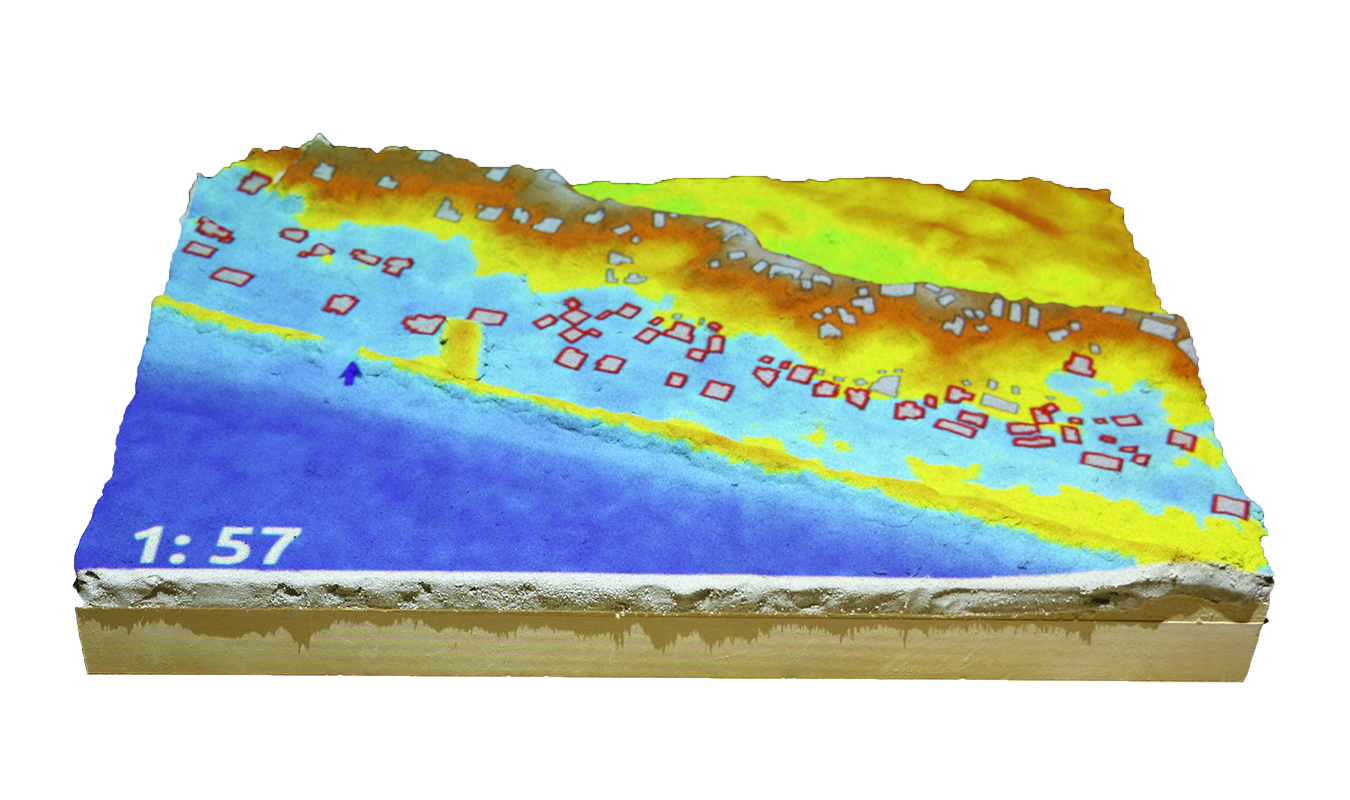
\includegraphics[trim={0 0 0 1cm},clip,width=\textwidth]{tl_coastal_4s.png}
                %\caption{The simulated flood and the houses lost}
        \end{subfigure}
        \caption{Serious gaming with Tangible Landscape: the coastal flooding game}
        \label{fig:coastal_game}
\end{figure}

%%%%%%%%%%%%%%%%%%%%%%%%%%%%%%%%%%%%%%

% how does the representation of spatial and temporal scale influence learning and decision-making?

\subsection{Understanding environmental processes}

Physical processes like the flow and dispersion of water are challenging to understand because they unfold in time and space, are historically contingent, are controlled by their context, and are driven by forces like gravity and momentum. The flow of water across a landscape is controlled by the morphological shape and gradient of the terrain. It is challenging to understand how water will flow across a landscape because one must not only understand how the shape and gradient of the terrain control the flow and dispersion of water locally, but also how water will flow between shapes and gradients – how the morphology is topologically connected. Understanding a physical process requires thinking at and across multiple spatial scales simultaneously. 

% tangible processes
Theoretically tangible interfaces for geographic information systems should help users understand environmental processes
by giving multidimensional data an interactive, physical form 
and
by graphically and sometimes even physically animating time, enabling users to explore temporal evolution and scale.

% spatial scale
With a physical model one can feel and cognitively grasp a range, albeit a limited range, of spatial scales 
-- scales ranging from what a fingertip can touch, what a hand can grasp, what a body can reach; 
the relationships between spatial scales within this range of motion 
should be naturally, subconsciously understood. 
%
Situating the spatial scale of a physical model  -- understanding how its modeled space relates to oneself, to experienced reality -- requires a reference, a common datum. 
%
Many natural features like topography \citep{Pelletier1996}, rivers \citep{Rodriguez-Iturbe1994,Tarboton1988}, and coastlines \citep{Mandelbrot1967} have fractal structures, are statistically self-similar, and are scale invariant over a range of spatial scales.
%
This can make is challenging to even approximately judge spatial scale from geographic features. 
Features of the built environment like houses, however, can be used to approximately judge scale 
using ones mental model of the feature as a reference. 
 %
Scales bars and scale rulers are commonly used to more precisely evaluate scale in maps, 
but are less useful with 3D physical models 
because it is challenging to read curvature, judge distance, and approximate size visually
\citep{Howard2012b,Howard2012c, Jeannerod1997}
and it is challenging to measure complex surfaces. 
%

Renderings such as perspective views of modeled landscape 
can help one imagine oneself in the landscape 
contextualizing the space,
relating it to personal experience,
and establishing relationships between the scale of the model and the scale of ones body. 
%
One can immerse oneself in the modeled landscape 
with stereoscopic 3D renderings 
using immersive technologies like virtual reality headsets 
or cave automatic virtual environments. 
%
While this may help one more richly experience the landscape
there is the risk of the `uncanny valley,' the cognitive dissonance 
when some aspects of the rendering look real, yet others look abstract \citep{Cafaro2014}. 
%
While renderings and immersive environments may help situate and contextualize the model
they would add such rich layers or streams of information 
that it may be challenging to focus on what is most useful at given moment. 
How can we limited our attention and select the most useful streams of information?

% shape displays
Shape displays -- tangible interfaces that physically represent surfaces or volumes like topography -- 
couple a physical model with a digital model
enabling users to kinaesthetically and computationally explore space. 
%
Continuous shape displays like Tangible Landscape precisely represent continuous surfaces or volumes, 
but are not scaleable. 
%
Dynamic, actuated shape displays like Relief \citep{Leithinger2010} are scaleable 
-- dynamically reconfiguring topography as one zooms across scales -- and physically animated, but discretely represent surfaces with 3D cells. The resolution of the surface, constrained by the mechanics of the actuators, cannot be high enough to give the impression of a continuous surface. 
%
Continuity is important because it links spatial scales. 
%
With continuous surfaces one can simultaneously think across spatial scales and potentially understand the topological connection between shapes.
%
With continuous surfaces one can simultaneously think across spatial scales.
One can see and feel the topological connection between shapes, 
potentially understanding the relationship between two spatial scales.
%
Continuous shape displays could be physically animated using robotic fabrication. 
The physical model could be dynamically reshaped by a robot 
using additive processes, subtractive processes, or casting. 
%
A dynamic, continuous shape display 
would physically, interactively animate time and space
in high resolution
so that complex processes can be intuitively grasped.
%
%With a dynamic, continuous shape display 
%that physically, interactively animates time and space in high resolution
%one should be able to naturally understand complex processes. 






%---------------------------------------------- BIBLIOGRAPHY ----------------------------------------------

\bibliographystyle{plainnat}
\bibliography{../tangible_topography} 
\end{document}








